\makeatletter % Use \makeatletter to make '@' a letter
\def\input@path{{../}} % Define input path to parent directory
\makeatother % Restore default category code of '@'

\documentclass[../main.tex]{subfiles}

\begin{document}

\section{Calculating the resummation coefficients}\label{sec:f_coeff}

In this section we discuss the calculation of the resummation coefficients $f_i(\lambda)$ for the thrust distribution.

In the article by Catani, Turnock, Webber and Trentadue \cite{CATANI1991491}, it was observed that 
for a final state configuration corresponding to a large value of thrust , \cref{eq:Thrust} can be approximated by

\begin{equation} \label{eq:Thrust_approx}
    \tau = 1-T \approx \frac{k_1^2+k_2^2}{Q^2}
\end{equation}

where $k_1^2$ and $k_2^2$ are the squared invariant masses of two back-to-back jets and $Q^2$ is the energy of the center of mass.
Thus the key to the evaluation of the thrust distributions is its relation to the quark jet mass distribution $J^q(Q^2,k^2)$, also denoted as $J^q_{k^2}(Q^2)$, which represents
the probability of finding a jet originating from quarks, with an invariant mass-squared $k^2$, produced in collisions with a center-of-mass energy $Q^2$.

Then the thrust distribution $R_T(\tau,\alpha_s(Q^2))$ \cref{eq:cumulative_distribution}
takes the form of a convolution of two jet mass distributions $J(Q^2,k_1^2)$ and $J(Q^2,k_2^2)$

\begin{equation}\label{eq:Thrust fraction convolution}
    R_T(\tau,\alpha_s(Q^2)) \underset{\tau \ll 1}{=} \int_0^\infty \dd k_1^2 \int_0^\infty  \dd k_2^2 J^q_{k_1^2}(Q^2) J^q_{k_2^2}(Q^2) \Theta\qty(\tau - \frac{k_1^2+k_2^2}{Q^2}) 
\end{equation}

Introducing the Laplace transform of the jet mass distribution:

\begin{equation}\label{eq:laplace_jet_mass}
    \Tilde{J}^q_\nu(Q^2) = \int_0^\infty J^q(Q^2,k^2) e^{-\nu k^2} \dd k^2 
\end{equation}

and using the integral representation of the Heaviside step function:

\begin{equation} \label{eq:heaviside_integral_representation}
    \Theta\qty(\tau - \frac{k_1^2+k_2^2}{Q^2}) = \frac{1}{2\pi i} \int_{C-i\infty}^{C+i\infty} \frac{\dd N}{N} e^{N \tau} e^{- N \frac{k_2^2+k_2^2}{Q^2}} 
\end{equation}

by substituting \cref{eq:heaviside_integral_representation} into \cref{eq:Thrust fraction convolution} and setting $N= \nu Q^2$ we obtain:

\begin{align}
    \begin{split} \label{eq:Thrust fraction}
    R_T(\tau) &= \int_{C - i \infty}^{C + i\infty} \frac{\dd N}{N} \frac{e^{N \tau}}{2\pi i} \qty[\int_0^\infty \dd k_1^2 e^{-\nu k_1^2} J^q_{k_1^2}(Q^2) ] \qty[\int_0^\infty \dd k_2^2 e^{-\nu k_2^2} J^q_{k_2^2}(Q^2)]\\
    &=\frac{1}{2\pi i}\int_{C - i \infty}^{C + i\infty} e^{N \tau} \qty[\Tilde{J}_\nu^q(Q^2)]^2 \frac{\dd N}{N}
    \end{split}
\end{align}

where $C$ is a real positive constant to the right of all singularities of the integrand $\Tilde{J}_\nu(Q^2)$ in the complex $\nu$ plane. 

An integral representation for the Laplace transform $\Tilde{J}_\nu(Q^2)$ is given by \cite{CATANI19933}:

\begin{equation}
    \ln \Tilde{J}_\nu^q(Q^2) = \int_0^1 \frac{\dd u}{u} \qty(e^{-u \nu Q^2}-1)\qty[ \int_{u^2 Q^2}^{u Q^2} \frac{1}{q^2} A\qty(\alpha_s(q^2)) \dd q^2 + \frac{1}{2} B\qty(\alpha_s(u Q^2))]
\end{equation}

with 

\begin{align*}
    A(\alpha_s) &= \sum_{n=1}^\infty A_n \qty(\frac{\alpha_s}{\pi})^n , & B(\alpha_s) &= \sum_{n=1}^\infty B_n\qty(\frac{\alpha_s}{\pi})^n .
\end{align*}

Function $A(\alpha_s)$ is associated with the cusp anomalous dimension and governs the exponentiation of the leading logarithms (LL). 
It captures the resummation of the soft and collinear gluon emissions that dominate in the limit of large thrust values.

Function $B(\alpha_S)$ includes the next-to-leading logarithmic (NLL) corrections and accounts for subleading contributions from hard collinear emissions.
It typically involves the non-cusp part of the anomalous dimensions and running of the coupling constant.

The integral as it is cannot be integrated, the $u$ integration may be performed using the prescription discussed in Appendix A of \cite{Catani_2003_appendix} and
readapting the formula to the case of Laplace transform instead of Mellin transform.

This method is a generalization of the prescription to NLL accuracy in \cite{CATANI19933}

\begin{equation}
    e^{-u \nu Q^2} - 1 \simeq -\Theta(u-v) \qq{with $v = \frac{N_0}{N}$}
\end{equation}

where $N_0 = e^{-\gamma_E}$.

In \cref{Appendix: Laplace and Mellin transform} we show that the prescription to evaluate the large-N Mellin moments of soft-gluon
contributins at an arbitrary logarithmic accuracy, can be used for the Laplace transform as well, then we can use this result to express \cref{eq:master formula} 
in an alternative representation:

\begin{equation}\label{eq:master_formula alt}
    \ln \Tilde{J}_\nu^q(Q^2) = - \int_{N_0/N}^{1} \frac{\dd u}{u} \qty[ \int_{u^2 Q^2}^{u Q^2} \frac{1}{q^2} A\qty(\alpha_s(q^2)) \dd q^2 + \frac{1}{2} \Tilde{B}\qty(\alpha_s(u Q^2))] + \ln \Tilde{C}\qty(\alpha_s(\mu^2),\frac{\mu^2}{Q^2}).
\end{equation}

Note that, due to the integration of the running coupling the integral in \cref{eq:master formula} is singular for all values of $N=\nu Q^2$. However, if we perform the integration up 
to a fixed logarithmic accuracy $N^kLL$ (\emph{i.e} we compute the leading $\alpha_s^n \ln^{n+1}N$, next-to-leading $\alpha_s^n \ln^nN$ and so on to $\alpha_s^n \ln^{n+1-k}$ terms ), we find the form factor: 

\begin{flalign}\label{eq:factorized_J_nu}
    \ln \Tilde{J}_\nu^q(Q^2) &= \ln N f_1(\lambda) + f_2(\lambda) + \alpha_s f_3(\lambda) + \alpha_s^2 f_4(\lambda) + \alpha_s^3 f_5(\lambda) + \order{\alpha_s^n \ln^{n-4}N} \nonumber\\
    &+ \ln \Tilde{C}\qty(\alpha_s(\mu^2),\frac{\mu^2}{Q^2})
\end{flalign}

From now on we'll always use \cref{eq:master_formula alt}, so i'll drop the $\Tilde{}$ notation for $B$.

We observe that the N-space formula \cref{eq:master_formula alt} is finite and uniquely defined up to the 
very large $N=N_L=\exp(\frac{1}{2\alpha_s b_0})$ ($\lambda = \frac{1}{2}$), thanks to the prescription above.


\subsection{resummation functions}

To calculate explicit expressions for the first few $f_i$ terms, we first write explicitly the internal integral of \cref{eq:master formula}, for
now let's forget the $\ln \Tilde{C}$ term, it can be absorbed into the definition of $A$ and $B$:

The $q^2$ integration also becomes simple if we use the renormalization group equation \cref{eq:RGE} to change
the integration variable to as

\begin{align}
    \frac{\dd q^2}{q^2} &= - \frac{\dd \alpha_s}{b_0 \alpha_s^2}\biggl(1-\frac{b_1}{b_0} \alpha_s  +  \frac{\left(b_1^2-b_2 b_0\right)}{b_0^2} \alpha_s^2 +\frac{ \left(-b_3 b_0^2  + 2 b_2  b_1 b_0-b_1^3\right)}{b_0^3} \alpha_s^3 & \nonumber\\
    &+\frac{ \left(-b_4 b_0^3  +  2 b_3 b_1 b_0^2 + b_2^2 b_0^2- 3 b_2 b_1^2 b_0 + b_1^4\right)}{b_0^4} \alpha_s^4 + \order{\alpha_s^5}\biggr)\\
    &= - \frac{\dd \alpha_s}{b_0 \alpha_s^2} ( N_0 + N_1 \alpha_s + N_2 \alpha_s^2 + N_3 \alpha_s^3 + N_4 \alpha_s^4 + \order{\alpha_s^5}) &\nonumber
\end{align}

where for convenience's sake we have defined:

\begin{align}
    N_0 &= 1 \qquad N_1 = \frac{b_1}{b_0} \qquad N_2 = \frac{\left(b_1^2-b_2 b_0\right)}{b_0^2} &\nonumber \\
    N_3 &= \frac{ \left(-b_3 b_0^2  + 2 b_2  b_1 b_0-b_1^3\right)}{b_0^3}  \\
    N_4 &= \frac{ \left(-b_4 b_0^3  +  2 b_3 b_1 b_0^2 + b_2^2 b_0^2- 3 b_2 b_1^2 b_0 + b_1^4\right)}{b_0^4} &\nonumber
\end{align}

Subsequently, the integral in \cref{eq:master_formula alt} can be expressed as:

\begin{flalign}
    &\int_{\alpha_s(u^2 Q^2)}^{\alpha_s(u Q^2)} \frac{\dd \alpha_s}{b_0 \alpha_s^2} ( N_0+ N_1 \alpha_s + N_2 \alpha_s^2 + N_3 \alpha_s^3 + N_4 \alpha_s^4) \sum_{n=1}^\infty A_n \qty(\frac{\alpha_s}{\pi})^n &\nonumber & \nonumber\\ 
    &= \int_{\alpha_s(u^2 Q^2)}^{\alpha_s(u Q^2)} \frac{\dd \alpha_s}{b_0} \biggl(\frac{A_1 N_0}{\pi \alpha_s} + \frac{\pi  A_1 N_1+A_2}{\pi ^2} + \frac{ \left(\pi  A_2 N_1+\pi ^2 A_1 N_2+A_3\right)}{\pi ^3} \alpha_s &\nonumber\\
    &+ \frac{ \left(\pi  A_3 N_1+\pi ^2 A_2 N_2+\pi ^3 A_1 N_3+A_4\right)}{\pi ^4}\alpha_s^2 \\ 
    &+ \frac{ \left(\pi  A_4 N_1+\pi ^2 A_3 N_2+\pi ^3 A_2 N_3+\pi ^4 A_1 N_4+A_5\right)}{\pi ^5} \alpha_s^3 +\order{\alpha_s^4}\biggr) & \nonumber
\end{flalign}

and keeping only terms up to $N_0$,$A_1$ and $\alpha_s^0$ we get contributions to $f_1$, keeping terms up to $N_1$,$A_2$ and $\alpha_s^1$ yields contributions to $f_2$ and so on. 
That's because after integration, we evaluate the integrand at $\alpha_s(u^2 Q^2)$ and $\alpha_s(u Q^2)$, where $\alpha_s$ is $\alpha_{\text{LO}}$ for $f_1$, $\alpha_{\text{NLO}}$ for $f_2$ and so on. 

And there's an easy way to see why it's like this, in fact it's also possible to do the $q^2$ integration directly, using \cref{eq:LO running coupling,eq:DNLO,eq:DNNLO,eq:DN3LO,eq:DN4LO} from \cref{sec:QCD_running_coupling}
and keeping in mind \cref{tab:contributions to different powers of alpha_s}.

\begin{flalign}
    &\int_{u^2 Q^2}^{u Q^2} \frac{\dd q^2}{q^2} \sum_{n=1}^\infty\frac{A_n}{\pi^n} \qty( \alpha_{\text{LO}}(q^2) + \delta\alpha_{\text{NLO}}(q^2) + \delta\alpha_{\text{NNLO}}(q^2) + \delta\alpha_{\text{N}^3\text{LO}}(q^2) + \delta\alpha_{\text{N}^4\text{LO}}(q^2) + \ldots)^n 
\end{flalign}

now we can see that if we consider terms up to $\alpha_s^1$ only $A_1$ contributes and this gives $f_1$, if we consider terms up to $\alpha_s^2$ we see $A_2$ starts to contribute together with $A_1  \delta\alpha_{\text{NLO}}$
and this gives $f_2$ , for $f_3$ we need to consider terms up to $\alpha_s^3$ and so on. 

For the $B$-term it's similar. However, since the $B$-term is "already integrated" in $q^2$, it contributes one order lower in $\alpha_s$ compared to the $A$-term. Specifically, $B_1$ starts to contribute from $f_2$, $B_2$ from $f_3$ and so on.  

Now armed with this knowledge we can calculate \cref{eq:master_formula alt} and find: 

\begingroup
\allowdisplaybreaks
\begin{equation}
    \ln \Tilde{J}_\nu^q(Q^2) = \ln N f_1(\lambda) + f_2(\lambda) + \alpha_s f_3(\lambda) + \alpha_s^2 f_4(\lambda) + \alpha_s^3 f_5(\lambda) + \order{\alpha_s^n \ln^{n-4}N}
\end{equation}

where $\lambda = \alpha_s b_0 \ln N$, $N=\nu Q^2$, $\alpha_s = \alpha_s(Q^2)$ and

\begin{flalign}\label{eq:f1}
    f_1(\lambda) =-\frac{A_1}{2 \pi  b_0 \lambda } \qty[(1-2 \lambda ) \ln (1-2 \lambda )-2 (1-\lambda ) \ln (1-\lambda )]
\end{flalign}


\begin{flalign}\label{eq:f2}
    f_2(\lambda) &= -\frac{A_2}{2 \pi ^2 b_0^2} \qty[2 \ln (1-\lambda )-\ln (1-2 \lambda )]+\frac{B_1 \ln (1-\lambda )}{2 \pi  b_0} +\frac{\gamma_E  A_1}{\pi  b_0} \qty[\ln (1-2 \lambda )-\ln (1-\lambda )] & \nonumber\\
    &-\frac{A_1 b_1}{2 \pi  b_0^3} \left[-\ln ^2(1-\lambda )+\frac{1}{2} \ln ^2(1-2 \lambda )-2 \ln (1-\lambda )+\ln (1-2 \lambda )\right]
\end{flalign}
    
\begin{flalign}\label{eq:f3}
    f_3(\lambda) &= -\frac{A_3 }{2 \pi ^3 b_0^2 (\lambda -1) (2 \lambda -1)}\lambda ^2 + \frac{B_2}{2 \pi ^2 b_0 (\lambda -1)}\lambda +\frac{B_2 \lambda }{2 \pi ^2 b_0 (\lambda -1)}& \nonumber\\
    &+\frac{b_1 A_2}{2 \pi ^2 b_0^3 (\lambda -1) (2 \lambda -1)} \left[3 \lambda ^2 + (1-\lambda) \ln (1-2 \lambda)- 2 (1-2 \lambda) \ln (1-\lambda)\right]& \nonumber \\
    &-\frac{\gamma_E A_2 \lambda }{\pi ^2 b_0 (\lambda -1) (2 \lambda -1)} - \frac{B_1 b_1 }{2 \pi  b_0^2 (\lambda -1)}\qty[\lambda +\ln (1-\lambda )] + \frac{\gamma_E B_1 \lambda}{2 \pi  (\lambda -1)}+\frac{\gamma_E ^2 A_1 \lambda  (2 \lambda -3)}{2 \pi  (\lambda -1) (2 \lambda -1)}& \nonumber \\ 
    &+ \frac{b_1 \gamma_E A_1}{\pi  b_0^2 (\lambda -1) (2 \lambda -1)}  \qty[-\lambda +(1-2 \lambda)  \ln (1-\lambda )- (1-\lambda)  \ln (1-2 \lambda )] \\
    &-\frac{b_1^2 A_1}{2 \pi  b_0^4 (\lambda -1) (2 \lambda -1)} \Bigl[\left(\lambda ^2+(2 \lambda -1) \ln (1-\lambda ) (2 \lambda +\ln (1-\lambda ))\right)&\nonumber\\
    &+\frac{1}{2}\left((1-\lambda) \ln ^2(1-2 \lambda )\right)-2 (\lambda -1) \lambda  \ln (1-2 \lambda )\Bigr] & \nonumber\\
    &-\frac{b_0 b_2 A_1}{2 \pi  b_0^4 (\lambda -1) (2 \lambda -1)} \left[\lambda ^2+ (\lambda -1) (2 \lambda -1)\qty(2 \ln (1-\lambda )+ \ln (1-2 \lambda ))\right] & \nonumber
\end{flalign}

\begin{flalign}\label{eq:f4}
    f_4(\lambda) &= -\frac{A_4 \lambda ^2 \left(2 \lambda ^2-6 \lambda +3\right)}{6 \pi ^4 b_0^2 (\lambda -1)^2 (2 \lambda -1)^2} + \frac{B_3 (\lambda -2) \lambda }{4 \pi ^3 b_0 (\lambda -1)^2} +\frac{b_1 A_3}{12 \pi ^3 b_0^3 (\lambda -1)^2 (2 \lambda -1)^2} \Bigl[15 \lambda ^2& \nonumber\\
    &+10 (\lambda -3) \lambda^3+3 (\lambda -1)^2 \ln (1-2 \lambda )-6 (1-2 \lambda )^2 \ln (1-\lambda )\Bigr]& \nonumber\\
    &+\frac{\gamma_E A_3 \lambda  (3 \lambda -2)}{2 \pi ^3 b_0 (\lambda -1)^2 (2 \lambda -1)^2}+\frac{\gamma_E B_2 (\lambda -2) \lambda }{2 \pi ^2 (\lambda -1)^2}-\frac{b_1 B_2 \left[\lambda ^2-2 \lambda -2 \ln (1-\lambda )\right]}{4 \pi ^2 b_0^2 (\lambda -1)^2} & \nonumber\\
    &+\frac{\gamma_E ^2 A_2 \lambda  \left(4 \lambda ^3-12 \lambda ^2+15 \lambda -6\right)}{2 \pi ^2 (\lambda -1)^2 (2 \lambda -1)^2}+\frac{b_1 \gamma_E A_2}{2 \pi ^2 b_0^2 (\lambda -1)^2 (2 \lambda -1)^2}  \Bigl[\lambda  (2-3 \lambda ) &\nonumber\\
    &+2 (\lambda -1)^2 \ln (1-2 \lambda )-2 (1-2 \lambda )^2 \ln (1-\lambda )\Bigr] +\frac{b_2 A_2 \lambda ^3 (4 \lambda -3)}{3 \pi ^2 b_0^3 (\lambda -1)^2 (2 \lambda -1)^2}& \nonumber\\
    &-\frac{b_1^2 A_2}{12 \pi ^2 b_0^4 (\lambda -1)^2 (2 \lambda -1)^2} \Bigl[\lambda ^2 \left(22 \lambda ^2-30 \lambda +9\right)+3 (\lambda -1)^2 \ln ^2(1-2 \lambda )&\nonumber\\
    &+3 (\lambda -1)^2 \ln (1-2 \lambda )-6 (1-2 \lambda )^2 \ln (1-\lambda ) (\ln (1-\lambda )+1)\Bigr] \\
    &+\frac{b_0 \gamma_E ^2 B_1 (\lambda -2) \lambda }{4 \pi  (\lambda -1)^2} +\frac{b_1 \gamma_E B_1 \ln (1-\lambda )}{2 \pi  b_0 (\lambda -1)^2} + \frac{b_2 B_1 \lambda ^2}{4 \pi  b_0^2 (\lambda -1)^2} & \nonumber\\
    &+ \frac{b_1^2 B_1 (\lambda -\ln (1-\lambda )) (\lambda +\ln (1-\lambda ))}{4 \pi  b_0^3 (\lambda -1)^2} +\frac{b_0 \gamma_E ^3 A_1 \lambda  \left(12 \lambda ^3-36 \lambda ^2+39 \lambda -14\right)}{6 \pi  (\lambda -1)^2 (2 \lambda -1)^2}& \nonumber\\
    &+\frac{b_1 \gamma_E ^2 A_1}{2 \pi  b_0 (\lambda -1)^2 (2 \lambda -1)^2} \left[2 (\lambda -1)^2 \ln (1-2 \lambda )-(1-2 \lambda )^2 \ln (1-\lambda )\right] &\nonumber\\
    &-\frac{b_1^2 \gamma_E A_1}{2 \pi  b_0^3 A_1 (\lambda -1)^2 (2 \lambda -1)^2} \left[(4 \lambda -3) \lambda ^2-(1-2 \lambda )^2 \ln ^2(1-\lambda )+(\lambda -1)^2 \ln ^2(1-2 \lambda )\right]&\nonumber\\
    &-\frac{b_1^3 A_1}{12 \pi  b_0^5 (\lambda -1)^2 (2 \lambda -1)^2} \Bigl[4 (3-4 \lambda ) \lambda ^3+2 (1-2 \lambda )^2 \ln (1-\lambda ) \left(\ln ^2(1-\lambda )-3 \lambda ^2\right)&\nonumber\\
    &+12 (\lambda -1)^2 \lambda ^2 \ln (1-2 \lambda )-(\lambda -1)^2 \ln ^3(1-2 \lambda )\Bigr] +\frac{b_2 \gamma_E A_1 \lambda ^2 (4 \lambda -3)}{2 \pi  b_0^2 (\lambda -1)^2 (2 \lambda -1)^2} & \nonumber\\
    &\frac{b_1 b_2 A_1}{12 \pi  b_0^4 (\lambda -1)^2 (2 \lambda -1)^2} \Bigl[\lambda ^2 (2 \lambda  (3-7 \lambda )+3)+3 \left(8 \lambda ^2-4 \lambda +1\right) (\lambda -1)^2 \ln (1-2 \lambda )&\nonumber\\
    &-6 (1-2 \lambda )^2 (2 (\lambda -1) \lambda +1) \ln (1-\lambda )\Bigr] + -\frac{b_3 A_1}{12 \pi  b_0^3 (\lambda -1)^2 (2 \lambda -1)^2} \Bigl[(2 (\lambda -3) \lambda +3) \lambda ^2&\nonumber\\
    &-6 \left(2 \lambda ^2-3 \lambda +1\right)^2 \ln (1-\lambda )+3 \left(2 \lambda ^2-3 \lambda +1\right)^2 \ln (1-2 \lambda )\Bigr] & \nonumber
\end{flalign}
    

\begin{flalign}\label{eq:f5}
    f_5(\lambda) &= -\frac{A_5 \lambda ^2 \left(4 \lambda ^4-18 \lambda ^3+33 \lambda ^2-24 \lambda +6\right)}{12 \pi ^5 b_0^2 (\lambda -1)^3 (2 \lambda -1)^3} + \frac{B_4 \lambda  \left(\lambda ^2-3 \lambda +3\right)}{6 \pi ^4 b_0 (\lambda -1)^3} \\ 
    &-\frac{\gamma_E A_4 \lambda  \left(7 \lambda ^2-9 \lambda +3\right)}{3 \pi ^4 b_0 (\lambda -1)^3 (2 \lambda -1)^3} +\frac{b_1 A_4}{36 \pi ^4 b_0^3 (\lambda -1)^3 (2 \lambda -1)^3} \Bigl[7 \lambda ^2 (\lambda  (\lambda  (2 \lambda  (2 \lambda -9)+33)-24)&\nonumber\\
    &+6)-6 (\lambda -1)^3 \ln (1-2 \lambda )+12 (2 \lambda -1)^3 \ln (1-\lambda )\Bigr] + \frac{\gamma_E B_3 \lambda  \left(\lambda ^2-3 \lambda +3\right)}{2 \pi ^3 (\lambda -1)^3}+  & \nonumber\\
    &\frac{b_1 B_3\left(\lambda ^3-3 \lambda ^2+3 \lambda +3 \ln (1-\lambda )\right)}{6 \pi ^3 b_0^2 (\lambda -1)^3} +\frac{\gamma_E ^2 A_3 \lambda  \left(8 \lambda ^5-36 \lambda ^4+66 \lambda ^3-69 \lambda ^2+39 \lambda -9\right)}{2 \pi ^3 (\lambda -1)^3 (2 \lambda -1)^3} & \nonumber\\
    &-\frac{b_1 \gamma_E A_3}{3 \pi ^3 b_0^2 (\lambda -1)^3 (2 \lambda -1)^3}  \Bigl[\lambda  ((9-7 \lambda ) \lambda -3)+3 (\lambda -1)^3 \ln (1-2 \lambda )&\nonumber\\
    &-3 (2 \lambda -1)^3 \ln (1-\lambda )\Bigr] +\frac{b_2 A_3\lambda ^3 \left(4 \lambda ^3-18 \lambda ^2+19 \lambda -6\right)}{4 \pi ^3 b_0^3 (\lambda -1)^3 (2 \lambda -1)^3}-& \nonumber\\
    &\frac{b_1^2 A_3}{36 \pi ^3 b_0^4 (\lambda -1)^3 (2 \lambda -1)^3} \Bigl[\lambda ^3(\lambda  (26 \lambda  (2 \lambda -9)+303)-150)-9 (\lambda -1)^3 \ln ^2(1-2 \lambda )&\nonumber\\
    &+24 \lambda^2 -6 (\lambda -1)^3 \ln (1-2 \lambda )+6 (2 \lambda -1)^3 \ln (1-\lambda ) (3 \ln (1-\lambda )+2)\Bigr] & \nonumber\\
    &+\frac{b_0 \gamma_E ^2 B_2 \lambda  \left(\lambda ^2-3 \lambda +3\right)}{2 \pi ^2 (\lambda -1)^3} -\frac{b_1 \gamma_E B_2 \ln (1-\lambda )}{\pi ^2 b_0 (\lambda -1)^3} +\frac{b_1^2 B_2 \left(\lambda ^3-3 \lambda ^2+3 \ln ^2(1-\lambda )\right)}{6 \pi ^2 b_0^3 (\lambda -1)^3}& \nonumber\\
    &-\frac{b_2 B_2 (\lambda -3) \lambda ^2}{6 \pi ^2 b_0^2 (\lambda -1)^3} + \frac{b_0 \gamma_E ^3 A_2 \lambda  \left(24 \lambda ^5-108 \lambda ^4+198 \lambda ^3-193 \lambda ^2+99 \lambda -21\right)}{3 \pi ^2 (\lambda -1)^3 (2 \lambda -1)^3} & \nonumber\\
    &+\frac{b_1^2 \gamma_E A_2}{3 \pi ^2 b_0^3 (\lambda -1)^3 (2 \lambda -1)^3} \Bigl[\lambda ^2 (\lambda  (18 \lambda -25)+9)+3 (\lambda -1)^3 \ln ^2(1-2 \lambda )&\nonumber\\
    &-3 (2 \lambda -1)^3 \ln ^2(1-\lambda )\Bigr] -\frac{b_2 \gamma_E A_2 \lambda ^2 \left(18 \lambda ^2-25 \lambda +9\right)}{3 \pi ^2 b_0^2 (\lambda -1)^3 (2 \lambda -1)^3} &\nonumber\\
    &+\frac{b_1^3 A_2}{36 \pi ^2 b_0^5 (\lambda -1)^3 (2 \lambda -1)^3} \Bigl[\lambda ^2 (\lambda  (\lambda  (2 \lambda  (50 \lambda -171)+339)-114)+6)&\nonumber\\
    &-6 (\lambda -1)^3 \ln ^3(1-2 \lambda )+12 (2 \lambda -1)^3 \ln (1-\lambda ) \left(-3 \lambda +\ln ^2(1-\lambda )+1\right)&\nonumber\\
    &+6 (6 \lambda -1) (\lambda -1)^3 \ln (1-2 \lambda )\Bigr]+\frac{b_3 A_2 \lambda ^3 \left(20 \lambda ^3-54 \lambda ^2+45 \lambda -12\right)}{12 \pi ^2 b_0^3 (\lambda -1)^3 (2 \lambda -1)^3} & \nonumber\\
    &-\frac{b_1 \gamma_E ^2 A_2}{\pi ^2 b_0 (\lambda -1)^3 (2 \lambda -1)^3} \Bigl[2 (\lambda -1)^3 \ln (1-2 \lambda )-(2 \lambda -1)^3 \ln (1-\lambda )\Bigr] & \nonumber\\
    &-\frac{b_2 b_1 A_2}{18 \pi ^2 b_0^4 (\lambda -1)^3 (2 \lambda -1)^3} \Bigl[\lambda ^2 (\lambda  (\lambda  (4 \lambda  (20 \lambda -63)+237)-75)+3)&\nonumber\\
    &+3 (6 \lambda -1) (\lambda -1)^3 \ln (1-2 \lambda )-6 (2 \lambda -1)^3 (3 \lambda -1) \ln (1-\lambda )\Bigr] & \nonumber \\
    &+\frac{b_0^2 \gamma_E ^3 B_1 \lambda  \left(\lambda ^2-3 \lambda +3\right)}{6 \pi  (\lambda -1)^3} -\frac{b_1^2 \gamma_E B_1  \left(\lambda -\ln ^2(1-\lambda )+\ln (1-\lambda )\right)}{2 \pi  b_0^2 (\lambda -1)^3}- & \nonumber\\
    &\frac{b_1^3 B_1}{12 \pi  b_0^4 (\lambda -1)^3}(\lambda +\ln (1-\lambda )) \left(2 \lambda ^2-3 \lambda +2 \ln ^2(1-\lambda )-2 \lambda  \ln (1-\lambda )-3 \ln (1-\lambda )\right) & \nonumber\\
    &+\frac{b_2 \gamma_E B_1 \lambda }{2 \pi  b_0 (\lambda -1)^3}-\frac{b_3 B_1 \lambda ^2 (2 \lambda -3)}{12 \pi  b_0^2 (\lambda -1)^3}+\frac{b_1 \gamma_E ^2 B_1 \left(\lambda ^3-3 \lambda ^2+3 \lambda -2 \ln (1-\lambda )\right)}{4 \pi  (\lambda -1)^3} & \nonumber\\
    &+\frac{b_2 b_1 B_1 \lambda  \left(2 \lambda ^2-3 \lambda -3 \ln (1-\lambda )\right)}{6 \pi  b_0^3 (\lambda -1)^3} +\frac{b_0^2 \gamma_E ^4 A_1}{12 \pi  (\lambda -1)^3 (2 \lambda -1)^3} \lambda  (2 \lambda -3) \Bigl[28 \lambda ^4 &\nonumber\\
    &-84 \lambda ^3+105 \lambda ^2-63 \lambda +15\Bigr] + \frac{b_1^3 \gamma_E A_1}{6 \pi  b_0^4 (\lambda -1)^3 (2 \lambda -1)^3} \Bigl[\lambda ^2 (4 \lambda  (3 (\lambda -3) \lambda +8)-9) &\nonumber\\
    &-2 (\lambda -1)^3 \ln ^3(1-2 \lambda )+3 (\lambda -1)^3 \ln ^2(1-2 \lambda )+12 \lambda  (\lambda -1)^3 \ln (1-2 \lambda ) &\nonumber\\
    &+(2 \lambda -1)^3 \ln (1-\lambda ) (\ln (1-\lambda ) (2 \ln (1-\lambda )-3) -6 \lambda )\Bigr] & \nonumber\\
    &+\frac{b_1^4 A_1}{24 \pi  b_0^6 (\lambda -1)^3 (2 \lambda -1)^3} \Bigl[8 (\lambda -1)^3 \lambda ^2 (4 \lambda -3) \ln (1-2 \lambda )&\nonumber\\
    &-2 (2 \lambda -1)^3 \ln (1-\lambda ) \left(2 (2 \lambda -3) \lambda ^2+\ln (1-\lambda ) ((\ln (1-\lambda )-2) \ln (1-\lambda )-6 \lambda )\right)&\nonumber\\
    &+2 \lambda ^3 \left(\lambda  \left(-28 \lambda ^2+54 \lambda -33\right)+6\right)+(\lambda -1)^3 \ln ^4(1-2 \lambda )-2 (\lambda -1)^3 \ln ^3(1-2 \lambda )- &\nonumber\\
    &12 (\lambda -1)^3 \lambda  \ln ^2(1-2 \lambda )\Bigr] -\frac{b_2 \gamma_E ^2 A_1 \lambda  \left(4 \lambda ^3-6 \lambda +3\right)}{2 \pi  b_0 (\lambda -1)^3 (2 \lambda -1)^3} +\frac{b_3 \gamma_E  \lambda ^2 \left(12 \lambda ^3-36 \lambda ^2+32 \lambda -9\right)}{6 \pi  b_0^2 (\lambda -1)^3 (2 \lambda -1)^3} & \nonumber\\
    &+\frac{b_2^2 A_1 }{36 \pi  b_0^4 (\lambda -1)^3 (2 \lambda -1)^3}\Bigl[\lambda ^2 (6-\lambda  (\lambda  (2 \lambda  (10 \lambda +9)-69)+42))&\nonumber\\
    &-12 \left(2 \lambda ^2-3 \lambda +1\right)^3 \ln (1-\lambda )+6 \left(2 \lambda ^2-3 \lambda +1\right)^3 \ln (1-2 \lambda )\Bigr] &\nonumber\\
    &+\frac{b_1^2 \gamma_E ^2 A_1}{2 \pi  b_0^2 (\lambda -1)^3 (2 \lambda -1)^3} \Bigl[\lambda  \left(4 \lambda ^3-6 \lambda +3\right)+2 (\lambda -1)^3 \ln ^2(1-2 \lambda )&\nonumber\\
    &-2 (\lambda -1)^3 \ln (1-2 \lambda )-(2 \lambda -1)^3 (\ln (1-\lambda )-1) \ln (1-\lambda )\Bigr] & \nonumber\\
    &-\frac{b_2 b_1^2 A_1}{36 \pi  b_0^5 (\lambda -1)^3 (2 \lambda -1)^3} \Bigl[\lambda ^2 (\lambda  (\lambda  (2 (153-82 \lambda ) \lambda -165)+12)+6)&\nonumber\\
    &-18 \lambda  (\lambda -1)^3 \ln ^2(1-2 \lambda )+6 \left(6 (1-2 \lambda )^2 \lambda -1\right) (\lambda -1)^3 \ln (1-2 \lambda )&\nonumber\\
    &-6 (2 \lambda -1)^3 \ln (1-\lambda ) \left(6 \lambda  (\lambda -1)^2-3 \lambda  \ln (1-\lambda )-2\right)\Bigr] & \nonumber \\
    &+\frac{b_1 \gamma_E ^3 A_1}{6 \pi  (\lambda -1)^3 (2 \lambda -1)^3} \Bigl[24 \lambda ^6-108 \lambda ^5+198 \lambda ^4-193 \lambda ^3 +16 \lambda ^3 \ln (1-\lambda ) &\nonumber\\
    &-8 \lambda ^3 \ln (1-2 \lambda )+99 \lambda ^2-24 \lambda ^2 \ln (1-\lambda )+24 \lambda ^2 \ln (1-2 \lambda )-21 \lambda &\nonumber\\
    &+12 \lambda  \ln (1-\lambda )-24 \lambda  \ln (1-2 \lambda )-2 \ln (1-\lambda )+8 \ln (1-2 \lambda )\Bigr] & \nonumber\\
    &-\frac{b_2 b_1 \gamma_E A_1}{3 \pi  b_0^3 (\lambda -1)^3 (2 \lambda -1)^3} \lambda  \Bigl[\lambda  (4 \lambda  (3 (\lambda -3) \lambda +8)-9)+6 (\lambda -1)^3 \ln (1-2 \lambda )&\nonumber\\
    &-3 (2 \lambda -1)^3 \ln (1-\lambda )\Bigr]+\frac{b_3 b_1 A_1}{18 \pi  b_0^4 (\lambda -1)^3 (2 \lambda -1)^3} \Bigl[\lambda ^3(\lambda  (4 (18-7 \lambda ) \lambda -51)+6) &\nonumber\\
    &+3 \lambda^2 +3 (2 \lambda  (\lambda  (8 \lambda -9)+3)-1) (\lambda -1)^3 \ln (1-2 \lambda )&\nonumber\\
    &-3 (2 \lambda -1)^3 (\lambda  (\lambda  (4 \lambda -9)+6)-2) \ln (1-\lambda )\Bigr] & \nonumber\\
    &-\frac{b_4 A_1}{36 \pi  b_0^3 (\lambda -1)^3 (2 \lambda -1)^3} \Bigl[\lambda ^2 (\lambda  (\lambda  (2 \lambda  (2 \lambda -9)+33)-24)+6)&\nonumber\\
    &-12 \left(2 \lambda ^2-3 \lambda +1\right)^3 \ln (1-\lambda )+6 \left(2 \lambda ^2-3 \lambda +1\right)^3 \ln (1-2 \lambda )\Bigr] & \nonumber
\end{flalign}

\endgroup

In \cref{eq:f3,eq:f4,eq:f5} we have removed some constant terms in order to make them homogeneous, \emph{i.e.} $f_i(0)=0$, those constant can be reabsorbed in the $C$-term \cref{eq:sigma}.

The functions $f_1(\lambda),f_2(\lambda)$ and $f_3(\lambda)$ were already known in the literature. Our results agree with those in \cite{CATANI19933,Aglietti:2005mb,Monni:2011gb} 
\footnote{We assume there is a misprint in $f_3(\lambda)$ in \cite{Monni:2011gb}, the last term proportional $A_1 \beta_1^2$ in parethesis should have a plus sign instead of
the minus sign.}.
In \cite{Aglietti:2005mb}, the resummation coefficients $f_i(\lambda)$ were derived from a similar integral but instead of Laplace space they're problem factorizes in
Mellin space, since in the large $N$ limit the Mellin and Laplace transforms are equivalent \cref{Appendix: Laplace and Mellin transform}, we obtain their same functional
form and thus compare our results.
In \cite{Monni:2011gb}, they applied Soft-Collinear Effective Theory (SCET) theory, in which contributions from Hard (H), Collinear (or Jet, J) and Soft (S) functions are treated separately
at their respective scales \cite{Becher_2008}: the hard scale of the $e^-e^+$  collision $ \mu_H \sim Q$, the invariant mass of the two back-to-back jets \cref{eq:Thrust_approx} $\mu_J^2 \sim k_1^2+k_2^2 \sim \tau Q^2$  and 
the soft scale $\mu_S \sim \frac{\mu_J^2}{\mu_H}\sim \tau Q$ . These functions are evaluated at their respective scales and then evolved to a common scale $\mu$ using renormalization group equations \cref{eq:RGE}.
The cross section is then factorized into a convolution of these functions and the resummation coefficients are obtained by performing the Laplace transform of the convolution.
The results of \cite{Monni:2011gb} are in agreement with our results; in fact their $f_1(\lambda)$ and $f_2(\lambda)$ are the same \footnote{The results differ by a factor 2 because we are considering the jet mass distribution, while the thrust distributions
is the convolution of two jet mass distributions \cref{eq:Thrust fraction convolution}.}
as the one originally obtained in \cite{CATANI19933}, however $f_3(\lambda)$ has two additional terms, one proportional to $c_s^{(1)}$ and the other to $c_j^{(1)}$ which we absorbed in the coefficients $A_3$ and $B_2$.

The functions $f_4(\lambda)$ and $f_5(\lambda)$, as far as we know they never appeared in the literature and are one the main results of the present work.

All the relevant constant can be found in \Cref{app:Ingredients}.
The coefficients $A_1,A_2$ and $B_1$ were already known in \cite{CATANI19933} and were obtained from the one and two loop splitting functions.
$A_3$ and $B_2$ were obtained by comparing our $f_3(\lambda)$ \cref{eq:f3} with the corresponding expression in Soft Collinear Effective Theory (SCET) \cite{Monni:2011gb} (Eq(4.17)) by 
absorbing the jet $c_J^{(1)}$ and soft $c_S^{(1)}$ terms into $A_3$ and $B_2$ terms.
We also compared our $G_{21}$ (in which $B_2$ appear) and $G_{32}$ (in which both $A_3$ and $B_2$ appear) with the exact expressions of 
$G_{21}$ and $G_{32}$ in \cite{Becher_2008} and found perfect agreement.

$B_3$ was extracted by comparing our $G_{31}$ in \Cref{app:Ingredients} with the exact expression of $G_{31}$ given by \cite{Monni:2011gb}.

Lastly $A_4, A_5$ and $B_4$ can be obtained by comparing $f_4(\lambda)$ and $f_5(\lambda)$ with the corresponding expression derived from \cite{Ju_2023} by incorporating the hard form factor 
of \cite{chakraborty2022hbbarbvertexloopshard} as appropriate, then absorbing contribution from the jet and soft functions into $A_4,A_5$ and $B_4$.

To obtain the Laplace trasform of the thrust distribution \cref{eq:Laplace transform distribution}, 
we perform the Laplace transform of the convolution \cref{eq:Thrust fraction convolution}.
By applying the convolution theorem, we find that it is twice the integral given by \cref{eq:master formula} that we have just calculated. 
Therefore, we multiply by 2 the $f_i(\lambda)$ we just obtained \cref{eq:f1,eq:f2,eq:f3,eq:f4,eq:f5}.

\begin{figure}[htbp]
    \centering
    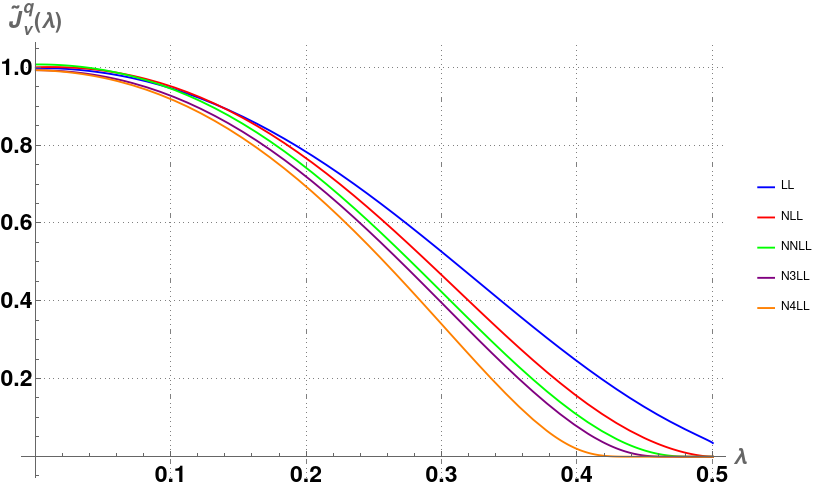
\includegraphics[width=\textwidth]{figures/Laplace_J_orders.png}
    \caption{Plot of $J_\nu^q$ function defined in \cref{eq:factorized_J_nu} at different logarithmin orders.}
    \label{fig:J_nu}
\end{figure}

\end{document}